%% Author: Leighton Pritchard
%% Copyright: James Hutton Institute
%% 2015-03-07: Slides for teaching at University of Dundee, 17th March 2015
%% This presentation was an invited lecture on comparative genomics and visualisation
%% for the BS32010 course.

%% UNCOMMENT FOR SLIDES
\documentclass[table]{beamer}
\mode<presentation>

%% UNCOMMENT FOR HANDOUTS
%\documentclass[handout]{beamer}
\usepackage{handoutWithNotes}
\pgfpagesuselayout{4 on 1 with notes}[a4paper,border shrink=5mm]

%% GENERIC STYLE SETTINGS BELOW
\usetheme{default}
\usepackage{listings}
\usepackage{multirow}
\usepackage{xcolor}
\usepackage{hyperref}
%\usepackage[multiple]{footmisc}

\usebackgroundtemplate{

\includegraphics[width=\paperwidth,height=\paperheight]{images/hutton_background}
}
%% PRESENTATION CONFIGURATION PARAMETERS %%%%%%%%%%%%%%%%%%%%%%%%%%%%%%%%%%%%%%%
%\titlebackgroundfile{images/hutton_title}
%\framebackgroundfile{images/hutton_background}
\definecolor{hutton_green}{HTML}{78A22F}
\definecolor{hutton_purple}{HTML}{872175}
\definecolor{hutton_blue}{HTML}{569BBE}
\definecolor{olive}{rgb}{0.3, 0.4, .1}
\definecolor{fore}{RGB}{249,242,215}
\definecolor{back}{RGB}{51,51,51}
\definecolor{title}{RGB}{255,0,90}
\definecolor{dgreen}{rgb}{0.,0.6,0.}
\definecolor{gold}{rgb}{1.,0.84,0.}
\definecolor{JungleGreen}{cmyk}{0.99,0,0.52,0}
\definecolor{BlueGreen}{cmyk}{0.85,0,0.33,0}
\definecolor{RawSienna}{cmyk}{0,0.72,1,0.45}
\definecolor{Magenta}{cmyk}{0,1,0,0}
\usefonttheme{structurebold}
\setbeamercolor{alerted text}{fg=orange}
\setbeamercolor{background canvas}{bg=white}
\setbeamercolor{block title}{bg=hutton_purple}
\setbeamercolor{frametitle}{fg=hutton_purple}
\setbeamercolor{title}{fg=black}
\setbeamercolor{titlelike}{fg=hutton_green}
\setbeamercolor{author}{fg=hutton_purple}
\setbeamercolor{author in head/foot}{fg=white}
\setbeamercolor{title in head/foot}{fg=white}
\setbeamercolor{section in head/foot}{fg=hutton_purple}
\setbeamercolor{normal text}{fg=black}
\setbeamercolor{frametitle}{fg=hutton_purple}
\setbeamerfont{block title}{size={}}
\setbeamerfont{author}{size=\footnotesize}
\setbeamerfont{institute}{size=\tiny}
\setbeamerfont{date}{size=\footnotesize}
\setbeamercolor{section in toc shaded}{fg=hutton_purple}
\setbeamercolor{section in toc}{fg=hutton_purple}
\setbeamercolor{subsection in toc shaded}{fg=hutton_purple}
\setbeamercolor{subsection in toc}{fg=hutton_purple}
\setbeamertemplate{itemize item}[circle]
\setbeamertemplate{itemize subitem}[circle]
\setbeamertemplate{itemize subsubitem}[circle]
\setbeamertemplate{itemize subsubsubitem}[circle]
\setbeamercolor{itemize item}{fg=hutton_purple}
\setbeamercolor{itemize subitem}{fg=hutton_purple}
\setbeamercolor{itemize subsubitem}{fg=hutton_purple}
\setbeamercolor{itemize subsubsubitem}{fg=hutton_purple}
\setbeamercolor{enumerate item}{fg=hutton_purple}
\setbeamercolor{enumerate subitem}{fg=hutton_purple}
\setbeamercolor{enumerate subsubitem}{fg=hutton_purple}
\setbeamercolor{enumerate subsubsubitem}{fg=hutton_purple}
\setbeamercolor{alerted text}{fg=hutton_green}
\setbeamerfont{alerted text}{series=\bfseries}
% This command makes sure that acrobat reader doesn't change the colours of the slide
% when there are figures with transparencies.
\pdfpageattr {/Group << /S /Transparency /I true /CS /DeviceRGB>>}

%Disables discrete bottom navigation bar
\beamertemplatenavigationsymbolsempty

% Modify the slide titles to avoid the corner images,
\setbeamertemplate{frametitle}
{
\vspace{0.05\textheight}
\noindent\quad\begin{minipage}[t][0.12\textheight][t]{0.85\textwidth}
\insertframetitle\par
\end{minipage}
}

% Modify title page to avoid the big logo on right
\setbeamertemplate{title page}{
    \begin{picture}(0,0)
            %This ends up on top of the default background image, rather than replacing it:
            \put(-30,-165){%
                
\includegraphics[width=\paperwidth,height=\paperheight]{images/hutton_title}
            }
            \put(0,-75){%
                \begin{minipage}[b][0.4\textheight][t]{0.75\textwidth}
                    \usebeamerfont{title}\usebeamercolor[fg]{title}{\inserttitle\par}
                    \usebeamerfont{subtitle}\usebeamercolor[fg]{subtitle}{\insertsubtitle\par}
                \end{minipage}
            }
            \put(0,-125){%
                \begin{minipage}[b][0.1\textheight][t]{\textwidth}
                    \usebeamerfont{author}\usebeamercolor[fg]{author}{\insertauthor\par}
                    \usebeamerfont{institute}\usebeamercolor[fg]{institute}{\insertinstitute\par}
                \end{minipage}
            }
    \end{picture}
}

% Make \verbatim environment tiny font
\makeatletter
\def\verbatim{\tiny\@verbatim \frenchspacing\@vobeyspaces \@xverbatim}
\makeatother

%%%%%%%%%%%%%%%%%%%%%%%%%%%%%%%%%%%%%%%%%%%%%%%%%%%%%%%%%%%%%%%%%%%%%%%%%%%%%%%%

% LISTINGS SETTING
% Settings for code listings in lstlistings

\definecolor{hutton_lightgreen}{HTML}{C8F27F}

\lstset{ %
  backgroundcolor=\color{hutton_lightgreen},   % choose the background color; you must add \usepackage{color} or \usepackage{xcolor}
  basicstyle=\tiny\ttfamily,        % the size of the fonts that are used for the code
  breakatwhitespace=false,         % sets if automatic breaks should only happen at whitespace
  breaklines=true,                 % sets automatic line breaking
  captionpos=b,                    % sets the caption-position to bottom
  commentstyle=\color{red},    % comment style
  deletekeywords={...},            % if you want to delete keywords from the given language
  escapeinside={\%*}{*)},          % if you want to add LaTeX within your code
  extendedchars=true,              % lets you use non-ASCII characters; for 8-bits encodings only, does not work with UTF-8
  frame=single,                    % adds a frame around the code
  keepspaces=true,                 % keeps spaces in text, useful for keeping indentation of code (possibly needs columns=flexible)
  keywordstyle=\color{blue},       % keyword style
%  language=Octave,                 % the language of the code
  morekeywords={*,...},            % if you want to add more keywords to the set
  numbers=left,                    % where to put the line-numbers; possible values are (none, left, right)
  numbersep=5pt,                   % how far the line-numbers are from the code
  numberstyle=\tiny\color{gray}, % the style that is used for the line-numbers
  rulecolor=\color{black},         % if not set, the frame-color may be changed on line-breaks within not-black text (e.g. comments (green here))
  showspaces=false,                % show spaces everywhere adding particular underscores; it overrides 'showstringspaces'
  showstringspaces=false,          % underline spaces within strings only
  showtabs=false,                  % show tabs within strings adding particular underscores
  stepnumber=1,                    % the step between two line-numbers. If it's 1, each line will be numbered
  stringstyle=\color{violet},     % string literal style
  tabsize=4,                       % sets default tabsize to 2 spaces
  title=\lstname                   % show the filename of files included with \lstinputlisting; also try caption instead of title
}


%%%
% TITLE PREAMBLE
\title[Comparative Genomics and Visualisation: 3.Whole Genomes] % (optional, only for long titles)
{Comparative Genomics and \\ Visualisation \\
BS32010 \\
3.Whole Genome Comparisons}
%\subtitle{}
\author[Pritchard] % (optional, for multiple authors)
{Leighton~Pritchard$^{1,2,3}$}
\institute[The James Hutton Institute] % (optional)
{
  $^{1}$Information and Computational Sciences,\\
  $^{2}$Centre for Human and Animal Pathogens in the Environment,\\
  $^{3}$Dundee Effector Consortium,\\
  The James Hutton Institute, Invergowrie, Dundee, Scotland, DD2 5DA
}
\date[17th March 2015] % (optional)
{17th March 2015}
\subject{Bioinformatics, Genomics, Bacteria, Sequencing, Microbiology, Microbes, Comparative Genomics, Visualisation}

%%%
% TOC
% Show table of contents, with current section highlighted,
% at the start of each section

%\AtBeginSection[]
%{
%  \begin{frame}
%    \frametitle{Table of Contents}
%    \tableofcontents[currentsection] %,hideallsubsections]
%  \end{frame}
%}

\AtBeginSubsection[]
{
  \begin{frame}
    \frametitle{Table of Contents}
    \tableofcontents[currentsection,currentsubsection] %,hideallsubsections]
  \end{frame}
}

%%%
% START DOCUMENT
\begin{document}

\frame[plain]{\titlepage}

%% use.tex
%% Author: Leighton Pritchard
%% Copyright: James Hutton Institute
%% These slides describe the acceptable use policy for these slides and
%% materials

%
\begin{frame}
  \frametitle{Acceptable Use Policy}
  Recording of this talk, taking photos, discussing the content using \\
  email, Twitter, blogs, etc. is permitted (and encouraged), \\
  providing distraction to others is minimised. \\[0.5cm]
  These slides will be made available on SlideShare. \\[0.5cm]
  \textbf{These slides, and supporting material including exercises, are available at \href{https://github.com/widdowquinn/Teaching-2015-03-17-UoD_compgenvis}{https://github.com/widdowquinn/Teaching-2015-03-17-UoD\_compgenvis}}
\end{frame}

%%%
% SECTION: Bulk genome comparisons
\section{Whole Genome Comparisons}
% SUBSECTION
% Whole genome comparisons
\subsection{Introduction}
%% whole_genome_comparison_intro.tex
%% Author: Leighton Pritchard
%% Copyright: James Hutton Institute
%% Whole genome comparison introduction slides

%
\begin{frame}
  \frametitle{Whole genome comparisons}
  \Large{
    \textcolor{olive}{
      \textbf{
      Comparisons of one whole or draft genome with another \\
      (or many others)
      }
    }
  }
\end{frame}

%
\begin{frame}
  \frametitle{Whole genome comparisons}
  Minimum requirement: \textbf{two genomes} \\
  \begin{itemize}
    \item \textcolor{hutton_green}{Reference Genome}
    \item \textcolor{hutton_blue}{Comparator Genome}
  \end{itemize}
  The experiment produces a comparative result \textcolor{hutton_purple}{\textit{that is dependent on the choice of genomes}}.
\end{frame}

%
\begin{frame}
  \frametitle{Whole genome comparisons}
  Experimental methods mostly involve direct or indirect DNA hybridisation \\
  \begin{itemize}
    \item \textcolor{hutton_green}{DNA-DNA hybridisation (DDH)}
    \item \textcolor{hutton_blue}{Comparative Genomic Hybridisation (CGH)}
    \item \textcolor{hutton_purple}{Array Comparative Genomic Hybridisation (aCGH)}    
  \end{itemize}
\end{frame}

%
\begin{frame}
  \frametitle{Whole genome comparisons}
  Analogously, \textit{in silico} methods mostly involve sequence alignment \\
  \begin{itemize}
    \item \textcolor{hutton_green}{Average Nucleotide Identity (ANI)}
    \item \textcolor{hutton_blue}{Pairwise genome alignment}
    \item \textcolor{hutton_purple}{Multiple genome alignment}    
  \end{itemize}
\end{frame}
% SUBSECTION
% DNA-DNA hybridisation
\subsection{DNA-DNA hybridisation and ANI}
%% ddh_expt.tex
%% Author: Leighton Pritchard
%% Copyright: James Hutton Institute
%% Experimental DNA-DNA hybridisation

%
\begin{frame}
  \frametitle{DNA-DNA hybridisation (DDH)
  \footnote{\tiny{\href{http://dx.doi.org/10.1016/S0168-6445(00)00040-1
}{Morell\'{o}-Mora \& Amann (2011) \textit{FEMS Microbiol. Rev.} doi:10.1016/S0168-6445(00)00040-1
}}}
  }
  Several similar methods based on the same principle
  \begin{columns}[T] 
    \column{.4\textwidth} 
      \begin{itemize}
        \item \textcolor{hutton_green}{Denature gDNA mixture for organisms $A$, $B$}
        \item \textcolor{hutton_blue}{Allow gDNA to anneal; hybrids result}
      \end{itemize}
    \column{.6\textwidth}
      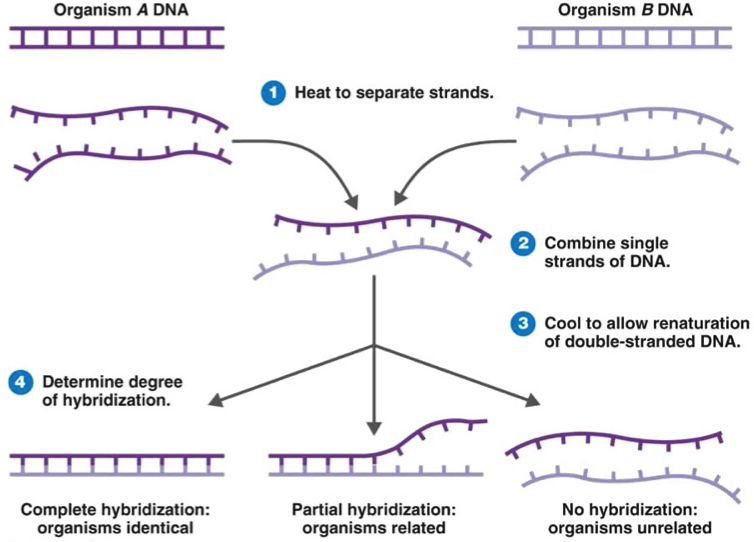
\includegraphics[width=\textwidth]{images/dna-dna_hyb}
  \end{columns}    
  Reassociation of gDNA $\approx$ sequence similarity
\end{frame}

%
\begin{frame}
  \frametitle{DNA-DNA hybridisation (DDH)
  \footnote{\tiny{\href{http://dx.doi.org/10.1016/S0168-6445(00)00040-1
}{Morell\'{o}-Mora \& Amann (2011) \textit{FEMS Microbiol. Rev.} doi:10.1016/S0168-6445(00)00040-1
}}}
  }
  \begin{columns}[T] 
    \column{.5\textwidth} 
      \begin{itemize}
        \item \textcolor{RawSienna}{Find homoduplex $T_{m1}$ for reference $A$}
        \item \textcolor{hutton_green}{Denature gDNA mixture for reference $A$, comparator $B$, and mix}
        \item \textcolor{hutton_green}{Allow gDNA to anneal; hybrids result}
        \item \textcolor{RawSienna}{Find heteroduplex $T_{m2}$ for mixture}
        \item \textcolor{hutton_blue}{$\Delta T_{m} = T_{m1} - T_{m2}$}        
        \item \textcolor{hutton_purple}{High $\Delta T \implies$ genomic difference (fewer H-bonds)}        
      \end{itemize}
    \column{.5\textwidth}
      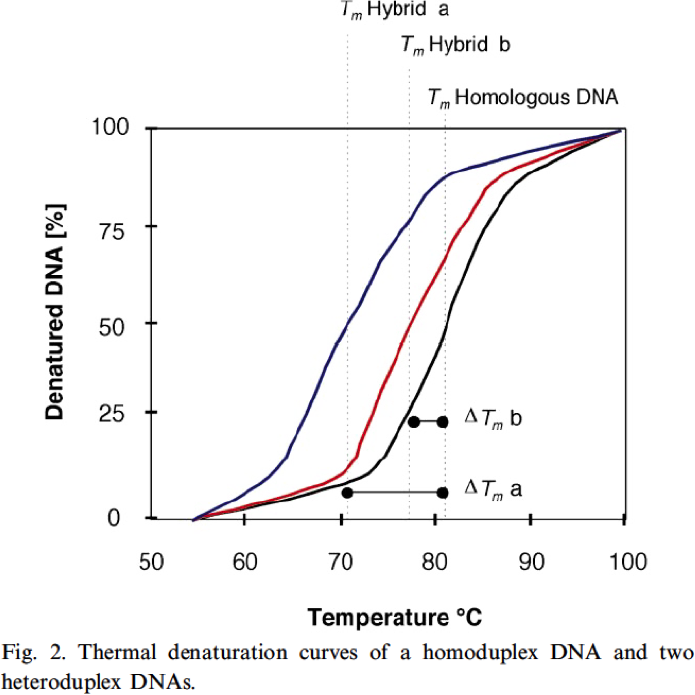
\includegraphics[width=\textwidth]{images/dna-dna_graph} \\
      \textcolor{red}{Proxy for sequence similarity}
  \end{columns}    
\end{frame}

%
\begin{frame}
  \frametitle{DNA-DNA hybridisation (DDH)
  \footnote{\tiny{\href{http://dx.doi.org/10.1007/BF02101980
}{Sibley \& Ahlquist (1984) \textit{J. Mol. Evol.} doi:10.1007/BF02101980
}}}  
  }
  Used for taxonomic classification in prokaryotes since '60s \\
  \textcolor{hutton_green}{Redefined accepted relationships for birds, primates in 1980s} \\
  \textcolor{RawSienna}{Controversial proof that \textit{Homo} shares more recent common ancestor with \textit{Pan} than with \textit{Gorilla}}
  \begin{center}
    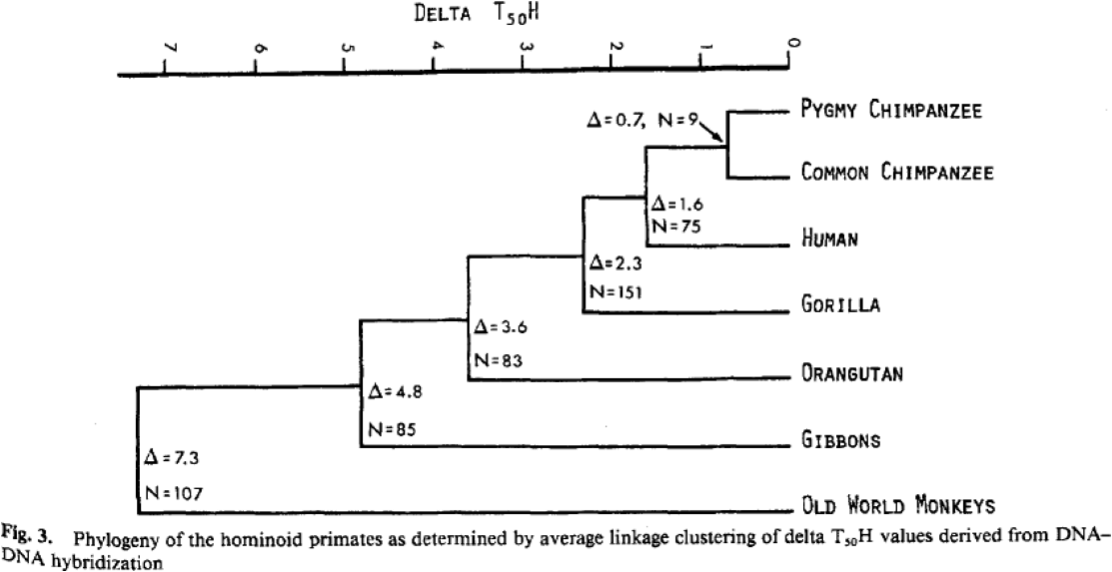
\includegraphics[width=0.9\textwidth]{images/dna-dna_primates} \\
  \end{center}  
\end{frame}

%
\begin{frame}
  \frametitle{DNA-DNA hybridisation (DDH)
  \footnote{\tiny{\href{http://dx.doi.org/10.1007/BF02101980
}{Sibley \& Ahlquist (1984) \textit{J. Mol. Evol.} doi:10.1007/BF02101980
}}}  
  \footnote{\tiny{\href{http://personal.uncc.edu/jmarks/DNAHYB/dnahyb2.html
}{http://personal.uncc.edu/jmarks/DNAHYB/dnahyb2.html
}}}  
  }
  \textcolor{RawSienna}{Controversial proof that \textit{Homo} shares more recent common ancestor with \textit{Pan} than with \textit{Gorilla}} 
  \begin{columns}[T] 
    \column{.6\textwidth} 
      \begin{itemize}
        \item \textcolor{hutton_green}{Allegations of data manipulation (see link $b$)}
        \item \textcolor{hutton_blue}{Close evolutionary relationships difficult to resolve due to $paralogy$}        
        \item \textcolor{hutton_purple}{Still the \textit{de facto} gold standard for microbiological taxonomic classification}        
      \end{itemize}
    \column{.4\textwidth}
      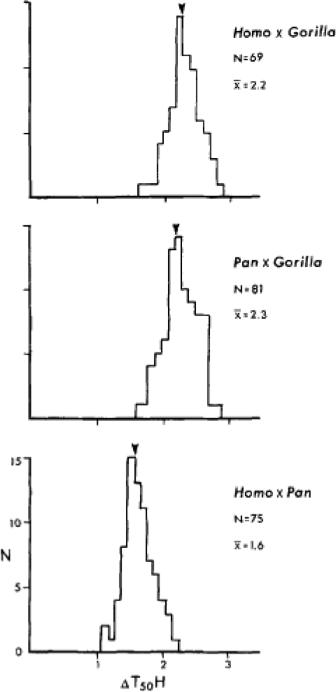
\includegraphics[width=0.6\textwidth]{images/dna-dna_controversy} \\
  \end{columns}    
\end{frame}
%% ani.tex
%% Author: Leighton Pritchard
%% Copyright: James Hutton Institute
%% Average Nucleotide Identity

%
\begin{frame}
  \frametitle{Average Nucleotide Identity (ANI)
  \footnote{\tiny{\href{http://dx.doi.org/10.1099/ijs.0.64483-0
}{Goris \textit{et al.} (2007) \textit{Int. J. System. Evol. Biol.} doi:10.1099/ijs.0.64483-0
}}}
  }
  Introduced as an \textit{in silico} substitute for DDH in 2007:
  \begin{columns}[T] 
    \column{.6\textwidth} 
      \begin{itemize}
        \item \textcolor{hutton_green}{70\% identity (DDH) = "gold standard" prokaryotic species boundary}
        \item \textcolor{hutton_blue}{70\% identity (DDH) $\approx$ 95\% identity (ANI)}
      \end{itemize}
    \column{.4\textwidth}
      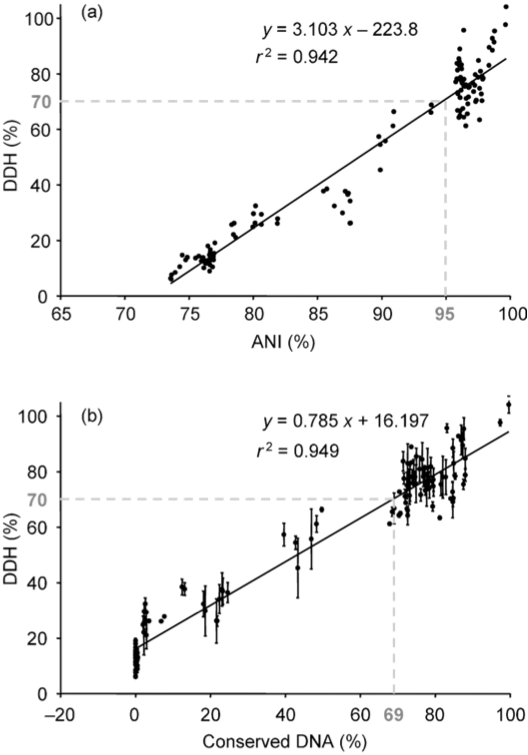
\includegraphics[width=\textwidth]{images/ani_ddh_equiv}
  \end{columns}    
\end{frame}

%
\begin{frame}
  \frametitle{Average Nucleotide Identity (ANI)
  \footnote{\tiny{\href{http://dx.doi.org/10.1099/ijs.0.64483-0
}{Goris \textit{et al.} (2007) \textit{Int. J. System. Evol. Biol.} doi:10.1099/ijs.0.64483-0
}}}
  }
  Original method emulated physical experiment:
  \begin{columns}[T] 
    \column{.6\textwidth} 
      \begin{enumerate}
        \item \textcolor{hutton_green}{break genome into 1020nt fragments}
        \item \textcolor{hutton_blue}{align all fragments with BLASTN}
        \item \textcolor{hutton_purple}{ANI = mean identity of all matches with $>30\%$ identity, $>70\%$ coverage}
      \end{enumerate}
    \column{.4\textwidth}
      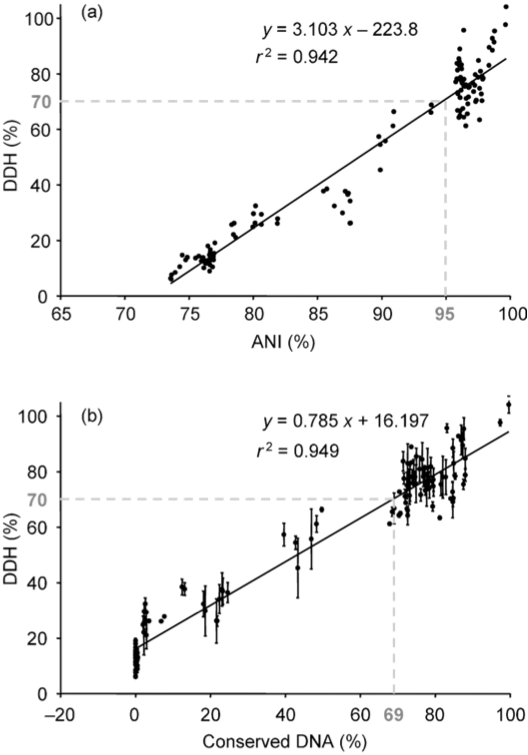
\includegraphics[width=\textwidth]{images/ani_ddh_equiv}
  \end{columns}    
\end{frame}

%
\begin{frame}
  \frametitle{Average Nucleotide Identity (ANI)
  \footnote{\tiny{\href{http://dx.doi.org/10.1073/pnas.0906412106
}{Richter \& Rossell\'{o}-M\'{o}ra \textit{et al.} (2009) \textit{Proc. Natl. Acad. Sci. USA} doi:10.1073/pnas.0906412106
}}}
  }
  ANIm and TETRA variants introduced in 2009:
  \begin{columns}[T] 
    \column{.5\textwidth} 
      \textcolor{RawSienna}{ANIm}
      \begin{enumerate}
        \item \textcolor{hutton_green}{Align sequences with NUCmer (no fragmentation)}
        \item \textcolor{hutton_purple}{ANI = mean identity of matches}
      \end{enumerate}
    \column{.5\textwidth}
      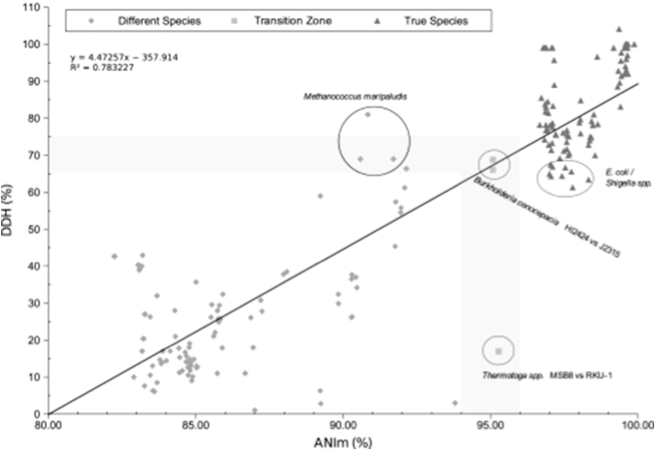
\includegraphics[width=\textwidth]{images/anim_ddh_equiv}
  \end{columns}    
  \textcolor{RawSienna}{TETRA}
  \begin{enumerate}
    \item \textcolor{hutton_green}{Calculate 4-mer frequencies}
    \item \textcolor{hutton_blue}{Determine Z-score for 4-mer deviation from expected value, given \%GC content}
    \item \textcolor{hutton_purple}{TETRA = Pearson correlation coefficient of Z-scores}
  \end{enumerate}
\end{frame}
% SUBSECTION
% Computational comparisons
\subsection{Experimental whole genome comparisons}
%% genome_comparisons_expt.tex
%% Author: Leighton Pritchard
%% Copyright: James Hutton Institute
%% In vitro experimental whole genome comparisons

%
\begin{frame}
  \frametitle{Comparative Genomic Hybridisation}
  \begin{itemize}
    \item Two genomes: \textcolor{RawSienna}{reference} and \textcolor{hutton_green}{test} fragmented \& labelled
    \item Hybridise \textcolor{RawSienna}{reference} and \textcolor{hutton_green}{test} against a third \textcolor{hutton_blue}{"normal"} genome.
  \end{itemize}
  \begin{center}
    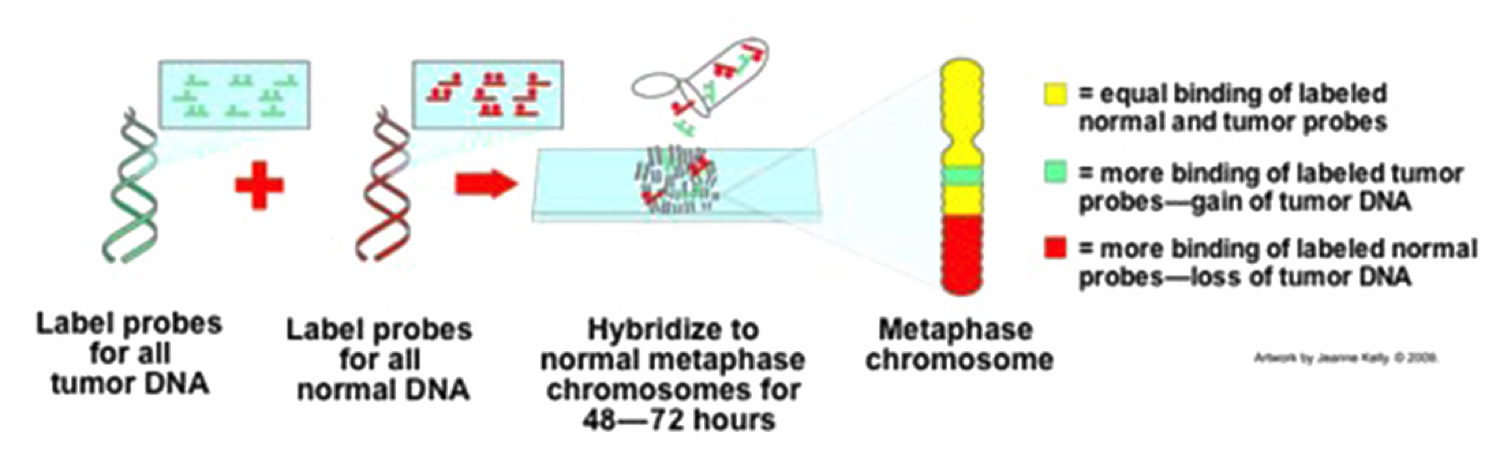
\includegraphics[width=\textwidth]{images/cgh}
  \end{center}  
  \begin{itemize}
    \item Differences in \textcolor{RawSienna}{red}/\textcolor{hutton_green}{green} intensity mapped by microscopy
    \item \textcolor{hutton_blue}{Colour intensity differences correspond to hybridisation, sequence similarity, and \textbf{copy number variations (CNV)}.}
    \item \textcolor{hutton_purple}{Can compare \textit{within} species/individuals (e.g. tumours), but labour-intensive, low-resolution}
  \end{itemize}  
\end{frame}

%
\begin{frame}
  \frametitle{CGH: epigenetics
  \footnote{\tiny{\href{http://dx.doi.org/10.1126/science.1359641
}{Kallionemi \textit{et al.} (1992) \textit{Science} doi:10.1099/10.1126/science.1359641
}}}
  \footnote{\tiny{\href{http://dx.doi.org/10.1073/pnas.0500398102
}{Fraga \textit{et al.} (2005) \textit{Proc. Natl. Acad. Sci. USA} doi:10.1073/pnas.0500398102
}}}
  }
  Measurements taken using image analysis - intensity on medial axis \\
  \textcolor{hutton_green}{Used for epigenetics: hybridisation of methylated DNA} \\
  \begin{columns}[T] 
    \column{.4\textwidth} 
      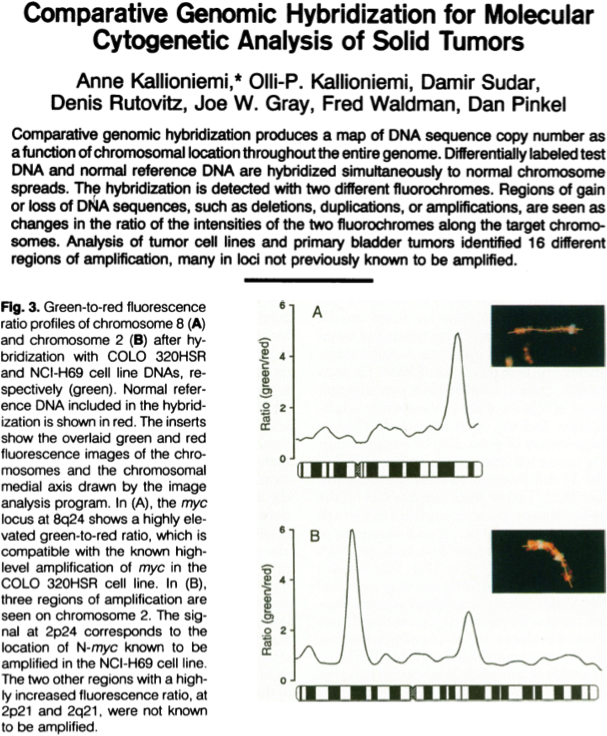
\includegraphics[width=\textwidth]{images/cgh_paper}
    \column{.4\textwidth}
      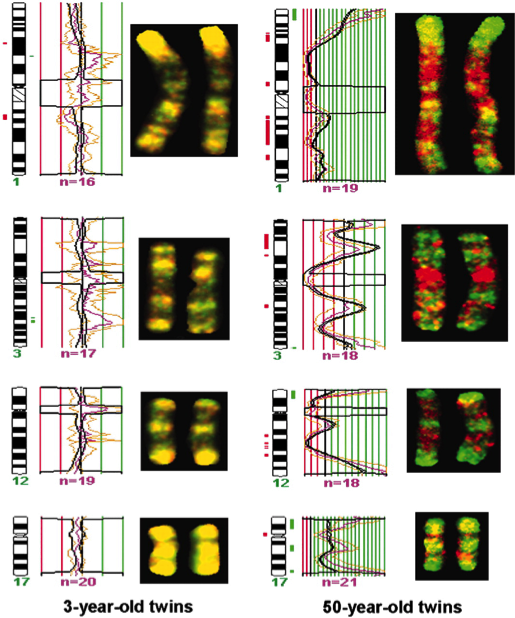
\includegraphics[width=\textwidth]{images/cgh_epigenetics}
  \end{columns}   
\end{frame}

%
\begin{frame}
  \frametitle{Array CGH (aCGH)
  \footnote{\tiny{\href{http://dx.doi.org/10.1038/12640
}{Pollack \textit{et al.} (1999) \textit{Nat. Genet.} doi:10.1099/10.1038/12640
}}}
  }
  Uses DNA microarrays: 1000s short, immobilised DNA probes \\
  gDNA, cDNA etc.\textcolor{RawSienna}{fluorescently}-\textcolor{hutton_green}{labelled} and hybridised to the array\\
  \begin{columns}[c] 
    \column{.4\textwidth} 
      \begin{itemize}
        \item Smaller sample sizes than CGH
        \item \textcolor{hutton_blue}{Automatable, high-throughput, high-resolution}
        \item \textcolor{hutton_purple}{Can identify copy number variation, segmental duplication, presence/absence}
      \end{itemize}
    \column{.6\textwidth}
      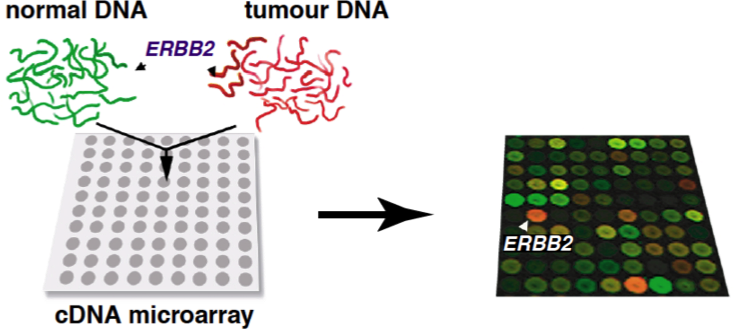
\includegraphics[width=\textwidth]{images/array_cgh}
  \end{columns}   
\end{frame}
\subsection{Pairwise genome sequence comparisons}
%% pairwise_genome_alignment.tex
%% Author: Leighton Pritchard
%% Copyright: James Hutton Institute
%% Pairwise genome alignment approaches

%
\begin{frame}
  \frametitle{Pairwise genome alignments}
  \textcolor{olive}{Genome sequence data gives much more detail and power} \\
  Pairwise comparisons require alignment of similar regions.
  \begin{center}
    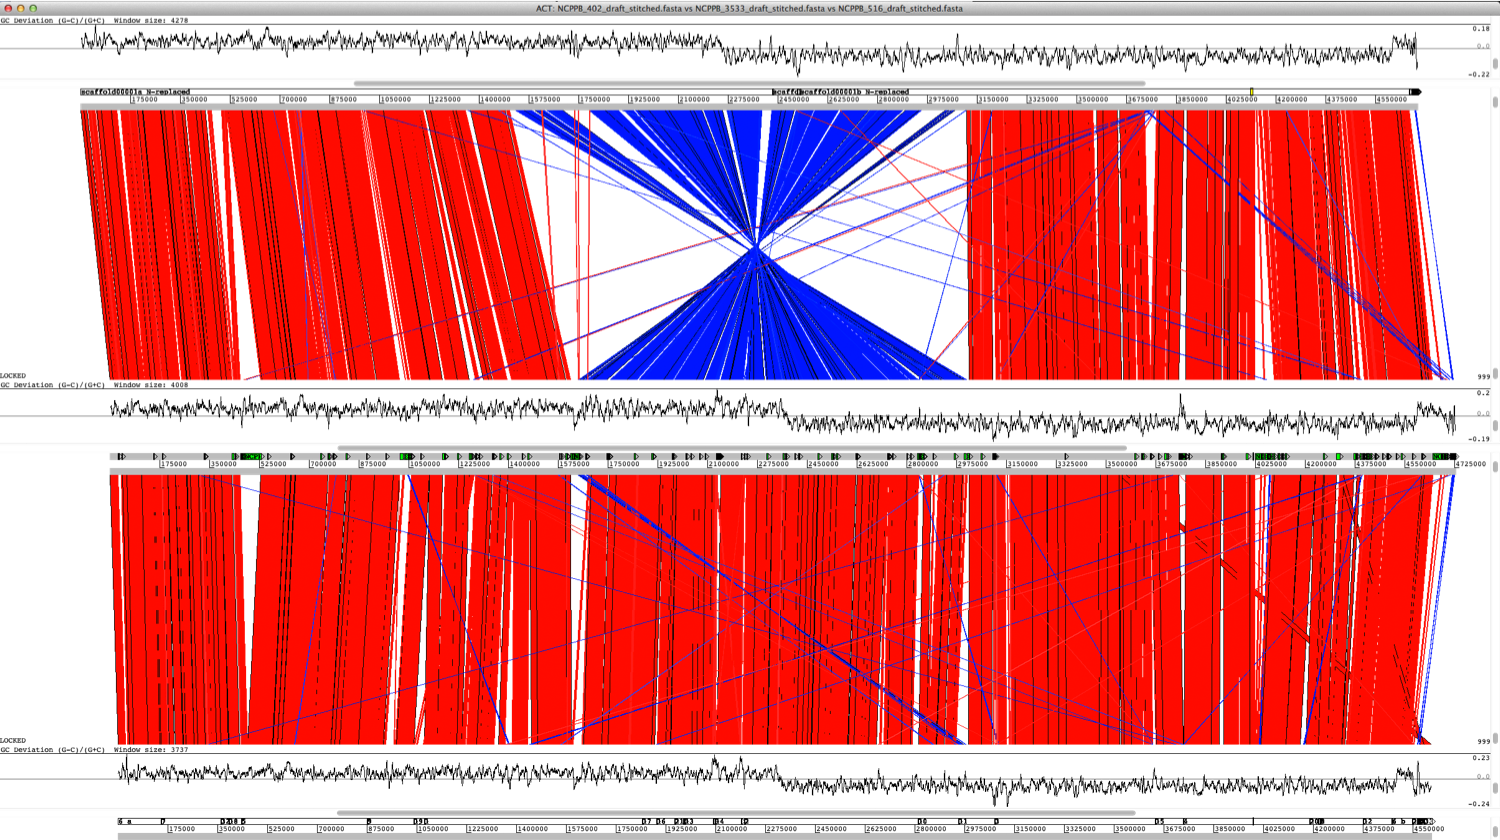
\includegraphics[width=\textwidth]{images/pairwise_genome_alignment}
  \end{center}  
\end{frame}

%
\begin{frame}
  \frametitle{Pairwise genome alignments}
  \textcolor{hutton_green}{Which genomes should you align (or not bother with)?} \\
  \textcolor{RawSienna}{For reasonable analysis, genomes should}:
  \begin{itemize}
    \item derive from a sufficiently \textcolor{red}{recent} common ancestor, so that \textcolor{hutton_purple}{homologous regions can be identified}
    \item derive from a sufficiently \textcolor{red}{distant} common ancestor, so that \textcolor{hutton_purple}{biologically meaningful changes are likely to be found}
  \end{itemize}
\end{frame}

%
\begin{frame}
  \frametitle{Alignment algorithms/programs}
  \textcolor{hutton_green}{I assume you're familiar with BLAST} \\
  (but, if not, see \url{supporting_information} subdirectory) \\~\\
  \textcolor{RawSienna}{Na\"{i}ve alignment algorithms are not appropriate}:
  \begin{itemize}
    \item Needleman-Wunsch: optimal global alignment
    \item Smith-Waterman: optimal local alignment
  \end{itemize}
  \textcolor{hutton_blue}{Cannot handle rearrangement} \\
  \textcolor{hutton_purple}{Computationally expensive}  
\end{frame}

%
\begin{frame}
  \frametitle{Alignment algorithms/programs}
  \textcolor{hutton_green}{Many whole-genome alignment algorithms proposed} \\
  Handle genome-scale evolutionary processes, scalable \\~\\
  \begin{itemize}
    \item \href{http://www.bx.psu.edu/~rsharris/lastz/}{LASTZ (http://www.bx.psu.edu/$\sim$rsharris/lastz/)}
    \item \href{http://genome.ucsc.edu/goldenPath/help/blatSpec.html}{\textcolor{hutton_blue}{\textbf{BLAT} (http://genome.ucsc.edu/goldenPath)}}
    \item \href{http://mugsy.sourceforge.net/}{Mugsy (http://mugsy.sourceforge.net/)}
    \item \href{http://www.ncbi.nlm.nih.gov/blast/html/megablast.html}{\textcolor{red}{\textbf{megaBLAST} (http://www.ncbi.nlm.nih.gov/blast/)}}
    \item \href{http://mummer.sourceforge.net/}{\textcolor{red}{\textbf{MUMmer} (http://mummer.sourceforge.net/)}}
    \item \href{http://lagan.stanford.edu/lagan_web/index.shtml}{{\textcolor{hutton_blue}{LAGAN (http://lagan.stanford.edu/lagan\_web/index.shtml)}}}
    \item WABA, etc?
  \end{itemize}
\end{frame}

%
\begin{frame}
  \frametitle{BLAT
  \footnote{\tiny{\href{http://dx.doi.org/10.1101/gr.229202
}{Kent (2002) \textit{Genome Res.} doi:10.1101/gr.229202
}}}
  }
  Broadly similar to BLAST \\~\\
  \textcolor{hutton_blue}{Main differences:}
  \begin{itemize}
    \item optimised to find \textcolor{hutton_purple}{only exact or near-exact matches} (speed)
    \item indexes the subject genome, and \textcolor{hutton_purple}{\textit{scans the query}}
    \item connects homologous match regions into a single alignment (BLAST reports these separately)
    \item reports mRNA match intron-exon bounds exactly (BLAST tends to extend beyond bounds)
  \end{itemize}
  \textcolor{hutton_green}{\textbf{ADVANTAGES}: fast, exact exon bounds, UCSC integration}
  \textcolor{RawSienna}{\textbf{DISADVANTAGES}: less sensitive on remote/divergent sequences}
\end{frame}

%
\begin{frame}
  \frametitle{megaBLAST
  \footnote{\tiny{Zhang \textit{et al.} (2000) \textit{J. Comp. Biol.} \textbf{7}(1-2): 203-214
}}
  \footnote{\tiny{Korf \textit{et al.} (2003) \textit{BLAST} O'Reilly \& Associates, Sebastopol, CA
}}
  }
  Optimised for:
  \begin{itemize}
    \item \textcolor{hutton_green}{speed and genome-level searching}
    \item \textcolor{hutton_blue}{queries on large sequence sets}: "query-packing"
    \item \textcolor{hutton_purple}{long alignments of very similar sequences} (\url{dc-megablast} for divergent sequences)
  \end{itemize}
  Uses Zhang et al. greedy algorithm, \textbf{not BLAST algorithm} \\~\\
  \textcolor{RawSienna}{BLASTN+ defaults to megaBLAST algorithm} \\
  (see \href{http://www.ncbi.nlm.nih.gov/blast/Why.shtml}{http://www.ncbi.nlm.nih.gov/blast/Why.shtml})
\end{frame}

%
\begin{frame}
  \frametitle{MUMmer
  \footnote{\tiny{\href{http://dx.doi.org/10.1186/gb-2004-5-2-r12
}{Kurtz \textit{et al.} (2004) \textit{Genome Biol.} doi:10.1186/gb-2004-5-2-r12
}}}
  }
  Conceptually completely different to BLAST/BLAT/megaBLAST \\
  \textcolor{RawSienna}{Uses \textit{suffix trees} for pattern matching}
  \begin{itemize}
    \item \textcolor{hutton_green}{Finds maximal exact matches}
    \item \textcolor{hutton_blue}{Memory use depends only on reference sequence size}
  \end{itemize}
  \begin{columns}[T] 
    \column{.5\textwidth} 
      \textcolor{hutton_purple}{Suffix Tree:}
      \begin{itemize}
        \item Constructed and searched in $O(n)$ time
        \item Useful algorithms are nontrivial
        \item \url{BANANA$}
      \end{itemize}
    \column{.5\textwidth}
      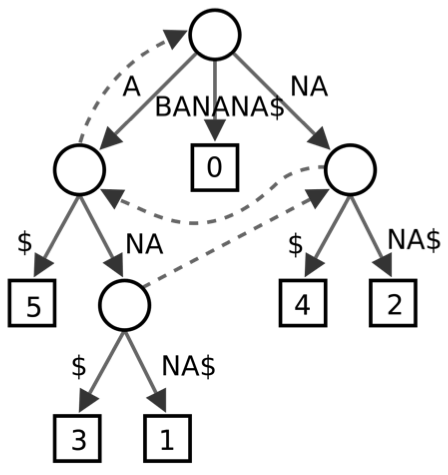
\includegraphics[width=0.75\textwidth]{images/suffix_tree}
  \end{columns}    
\end{frame}

%
\begin{frame}
  \frametitle{MUMmer
  \footnote{\tiny{\href{http://dx.doi.org/10.1186/gb-2004-5-2-r12
}{Kurtz \textit{et al.} (2004) \textit{Genome Biol.} doi:10.1186/gb-2004-5-2-r12
}}}
  }
  \textcolor{RawSienna}{Process:}
  \begin{enumerate}
    \item \textcolor{hutton_green}{Identify non-overlapping set of maximal exact matches (MUMs: \textit{maximal unique matches})}
    \item \textcolor{hutton_blue}{Cluster MUMs into \textit{alignment anchors}}
    \item \textcolor{hutton_purple}{Extend between anchors to produce final (gapped) alignment}    
  \end{enumerate}
  \textcolor{RawSienna}{The approach is very flexible}
  \begin{enumerate}
    \item Used in a suite of programs (\url{mummer}, \url{nucmer}, \url{promer}, $\ldots$)
    \item Nucleotide and "conceptual protein" (sensitive!) alignments
    \item Used for comparisons, scaffolding, repeat detection
    \item Basis of other aligners and assemblers, (\url{Mugsy}, \url{AMOS}, $\ldots$)
  \end{enumerate}
\end{frame}

%
\begin{frame}
  \frametitle{Whole genome comparisons}
  \Large{
    \textcolor{hutton_blue}{
      \textbf{
      EXERCISE 4: \\
      {\small \href{https://github.com/widdowquinn/Teaching-2015-03-17-UoD_compgenvis/blob/master/exercises/whole_genome_alignment/whole_genome_alignments_A.md}{\texttt{whole\_genome\_alignment/whole\_genome\_alignments\_A.md}}}
      }
    }
  }
\end{frame}


\subsection{Multiple genome sequence comparisons}
%% multiple_genome_alignment.tex
%% Author: Leighton Pritchard
%% Copyright: James Hutton Institute
%% Multiple genome alignment approaches

%
\begin{frame}
  \frametitle{Multiple genome alignments}
  \textcolor{olive}{Multiple genome alignments are ``harder'' than pairwise} \\
  \begin{itemize}
    \item Computationally difficult to produce
    \item \textcolor{red}{Lead to NP-complete optimisation problems!}
  \end{itemize}  
  \textcolor{hutton_green}{Solutions:} \textbf{heuristics}
  \begin{itemize}
    \item Progressive (build a tree, combine pairwise alignments)
    \item Iterative (realign initial sequences as new genomes added)
    \item \textcolor{hutton_blue}{Positional homology}
    \item \textcolor{hutton_purple}{\textit{Glocal} alignments}
  \end{itemize}  
\end{frame}

%
\begin{frame}
  \frametitle{Multiple genome alignment}
  Many tools either positional homology or glocal alignment
  \begin{columns}[T] 
    \column{.5\textwidth} 
      \textcolor{olive}{Several tools:}
      \begin{itemize}
        \item Mugsy: {\tiny\href{http://mugsy.sourceforge.net/}{(http://mugsy.sourceforge.net/)}}
        \item \textcolor{hutton_blue}{MLAGAN: {\tiny\href{http://lagan.stanford.edu/lagan_web/index.shtml}{(http://lagan.stanford.edu/lagan\_web/index.shtml)}}}
        \item TBA/MultiZ: {\tiny\href{http://www.bx.psu.edu/miller_lab/}{(http://www.bx.psu.edu/miller\_lab/)}}
        \item \textcolor{red}{\textbf{Mauve}: {\tiny\href{http://gel.ahabs.wisc.edu/mauve/}{(http://gel.ahabs.wisc.edu/mauve/)}}}
      \end{itemize}
    \column{.5\textwidth}
      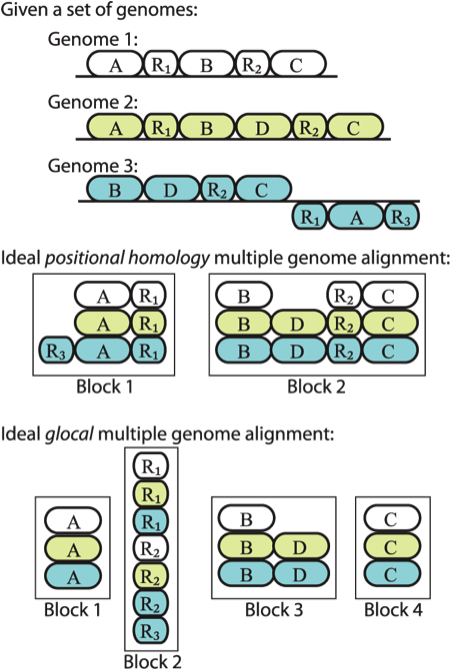
\includegraphics[width=0.75\textwidth]{images/poshom_v_glocal}
  \end{columns}    
\end{frame}

%
\begin{frame}
  \frametitle{LAGAN
  \footnote{\tiny{\href{http://dx.doi.org/10.1101/gr.926603
}{Brudno \textit{et al.} (2003) \textit{Genome Res.} doi:10.1101/gr.926603
}}}
  }
  Rapid pairwise alignment of homologous genomes
  \begin{columns}[T] 
    \column{.55\textwidth} 
      \textcolor{olive}{Algorithm:}
      \begin{enumerate}
        \item \textcolor{hutton_green}{Generate local alignments {\small(\textit{anchors}, B)}}
        \item \textcolor{hutton_blue}{Construct rough global map {\small(\textit{max-scoring ordered subset}, C)}}
        \item Join anchors that lie within a threshold distance
        \item \textcolor{hutton_purple}{Compute global alignment within each anchor {\small(\textit{Needleman-Wunsch}, D)}}
      \end{enumerate}
    \column{.45\textwidth}
      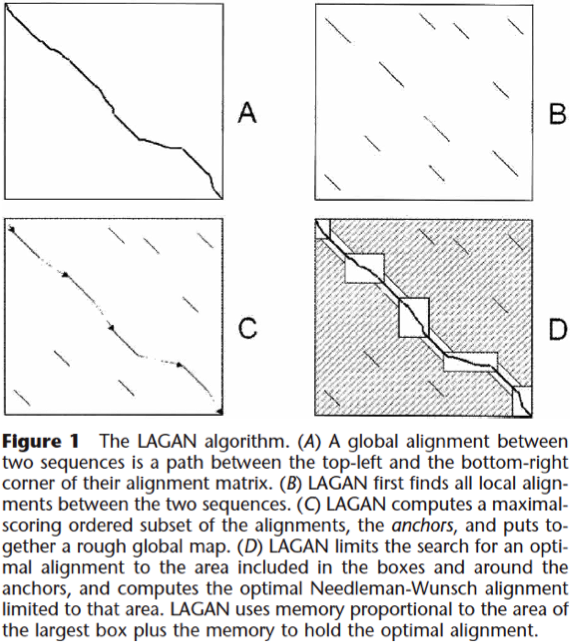
\includegraphics[width=\textwidth]{images/lagan_method}
  \end{columns}    
\end{frame}

%
\begin{frame}
  \frametitle{MLAGAN
  \footnote{\tiny{\href{http://dx.doi.org/10.1101/gr.926603
}{Brudno \textit{et al.} (2003) \textit{Genome Res.} doi:10.1101/gr.926603
}}}
  }
  Multiple genome alignment of $k$ genomes in $k-1$ alignment steps \\
  Progressive/iterative, using phylogenetic tree (like \texttt{CLUSTAL})
  \begin{columns}[T] 
    \column{.55\textwidth} 
      \textcolor{olive}{Algorithm:}
      \begin{enumerate}
        \item \textcolor{hutton_green}{Construct rough global maps between each pair of sequences {\small(step C in LAGAN)}}
        \item \textcolor{hutton_blue}{Progressive multiple alignment with anchors:}
		\begin{itemize}
          \item \textcolor{hutton_purple}{LAGAN alignment between closest pair of sequences: combined as \textit{multi-sequences}}
          \item \textcolor{hutton_purple}{Find rough global maps of this multi-sequence to all other multi-sequences}          
        \end{itemize}
      \end{enumerate}
    \column{.45\textwidth}
      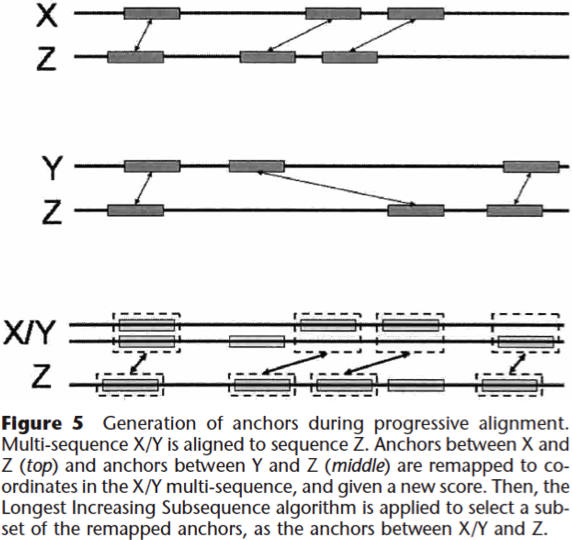
\includegraphics[width=\textwidth]{images/mlagan_method}
  \end{columns}    
\end{frame}

%
\begin{frame}
  \frametitle{Human:Mouse:Rat}
  \begin{center}
    
\includegraphics[height=0.7\textheight]{images/mouse-rat-photo}
  \end{center}
\end{frame}

%
\begin{frame}
  \frametitle{Human:Mouse:Rat
  \footnote{\tiny{\href{http://dx.doi.org/10.1101/gr.2067704
}{Brudno \textit{et al.} (2004) \textit{Genome Res.} doi:10.1101/gr.2067704
}}}
  }
  \textcolor{hutton_green}{Three-way progressive alignment} 
  \begin{columns}[T] 
    \column{.4\textwidth} 
    \textcolor{hutton_blue}{Initial alignments: BLAT \\
    Synteny: LAGAN/MLAGAN \\~\\}
    \textcolor{hutton_purple}{Three-way synteny}
      \begin{itemize}
        \item Homologous (HMR)
        \item Rodent-only (MR)
        \item Human-mouse (HM)
        \item Human-rat (HR)
      \end{itemize}
    \column{.6\textwidth}
      \begin{center}
        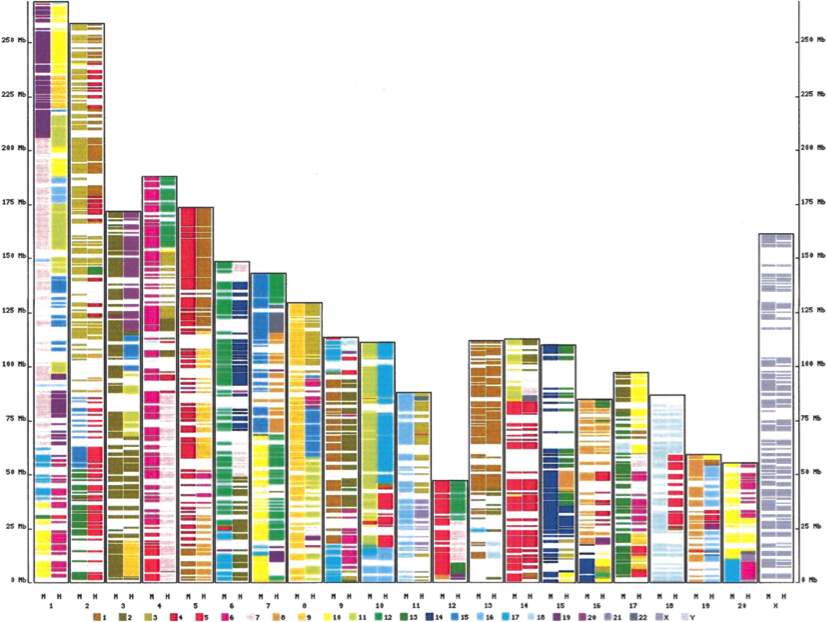
\includegraphics[width=\textwidth]{images/hmr_alignment} \\
        {\tiny(synteny mapped to rat genome)}
      \end{center}
  \end{columns}    
\end{frame}

%
\begin{frame}
  \frametitle{MAUVE
  \footnote{\tiny{\href{http://dx.doi.org/10.1101/gr.2289704
}{Darling \textit{et al.} (2003) \textit{Genome Res.} doi:10.1101/gr.2289704
}}}
  }
  MAUVE/Progressive MAUVE: \href{http://gel.ahabs.wisc.edu/mauve/}{http://gel.ahabs.wisc.edu/mauve/} \\
  \begin{columns}[T] 
    \column{.55\textwidth} 
      \textcolor{RawSienna}{Algorithm:}
      \begin{enumerate}
        \item \textcolor{hutton_green}{Find local alignments (\textit{multi-MUMs}, A)}
        \item Build guide tree from multi-MUMs
        \item \textcolor{hutton_blue}{Select subset of multi-MUMs (\textit{anchors}, B)}
        \begin{itemize}
          \item Partition into \textit{local collinear blocks} (LCBs)
        \end{itemize}
        \item \textcolor{hutton_purple}{Recursive anchoring to refine anchors (C)}
        \item Progressive alignment against guide tree
      \end{enumerate}
    \column{.45\textwidth}
      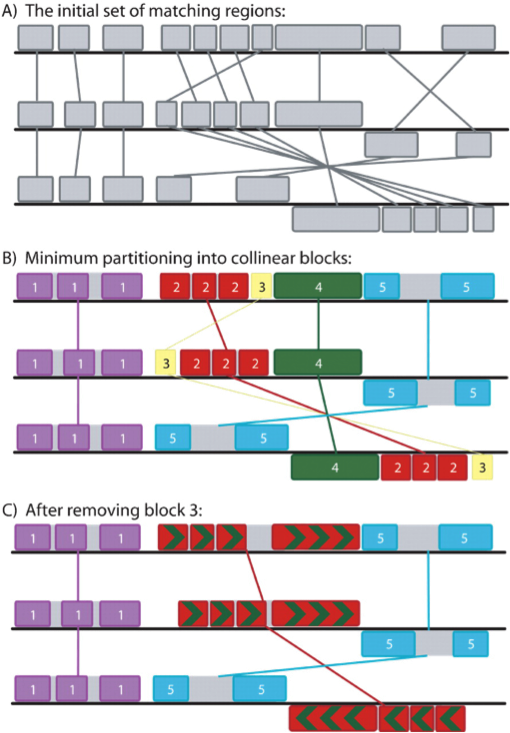
\includegraphics[width=0.9\textwidth]{images/mauve_method}
  \end{columns}    
\end{frame}

%
\begin{frame}
  \frametitle{MAUVE
  \footnote{\tiny{\href{http://dx.doi.org/10.1101/gr.2289704
}{Darling \textit{et al.} (2003) \textit{Genome Res.} doi:10.1101/gr.2289704
}}}
  }
  MAUVE alignment of LCBs in nine enterobacterial genomes \\
  \textcolor{hutton_green}{Evidence for rearrangement of homologous backbone sequence}
  \begin{center}
    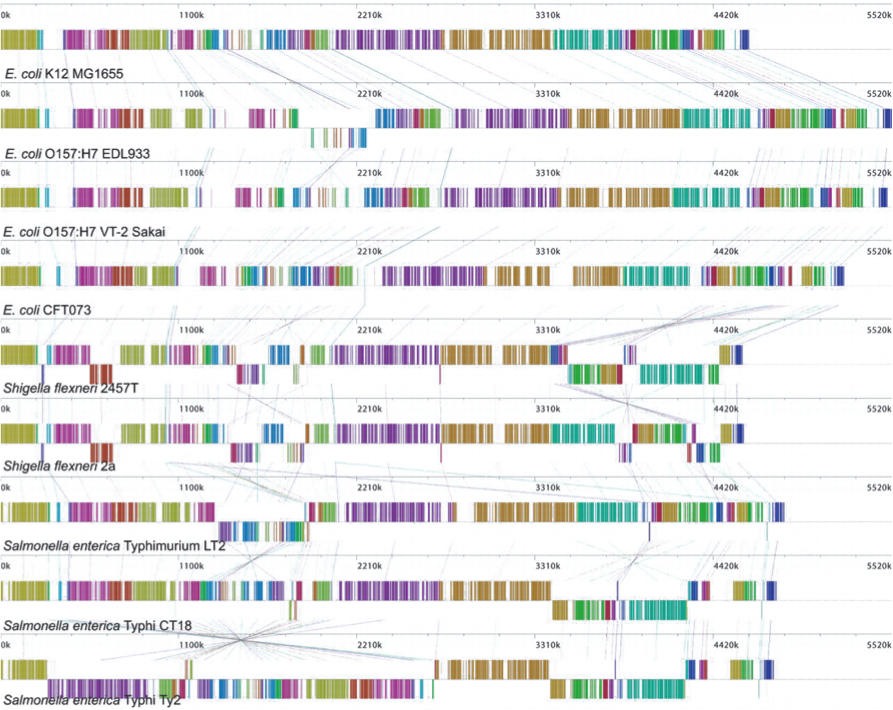
\includegraphics[height=0.6\textheight]{images/mauve_entero}
  \end{center}    
\end{frame}

%
\begin{frame}
  \frametitle{Draft genome alignment}
  \textcolor{olive}{High-throughput genome assemblies may be fragments (contigs)} \\
  Contigs can be ordered (\textit{scaffolded}):
  \begin{itemize}
    \item \textcolor{hutton_blue}{without alignment}, by long or paired-end reads
    \item \textcolor{hutton_purple}{by alignment}, to complete \textit{reference} genomes
    \item \textcolor{hutton_purple}{by alignment}, to other draft incomplete genomes
  \end{itemize}
  \begin{center}
    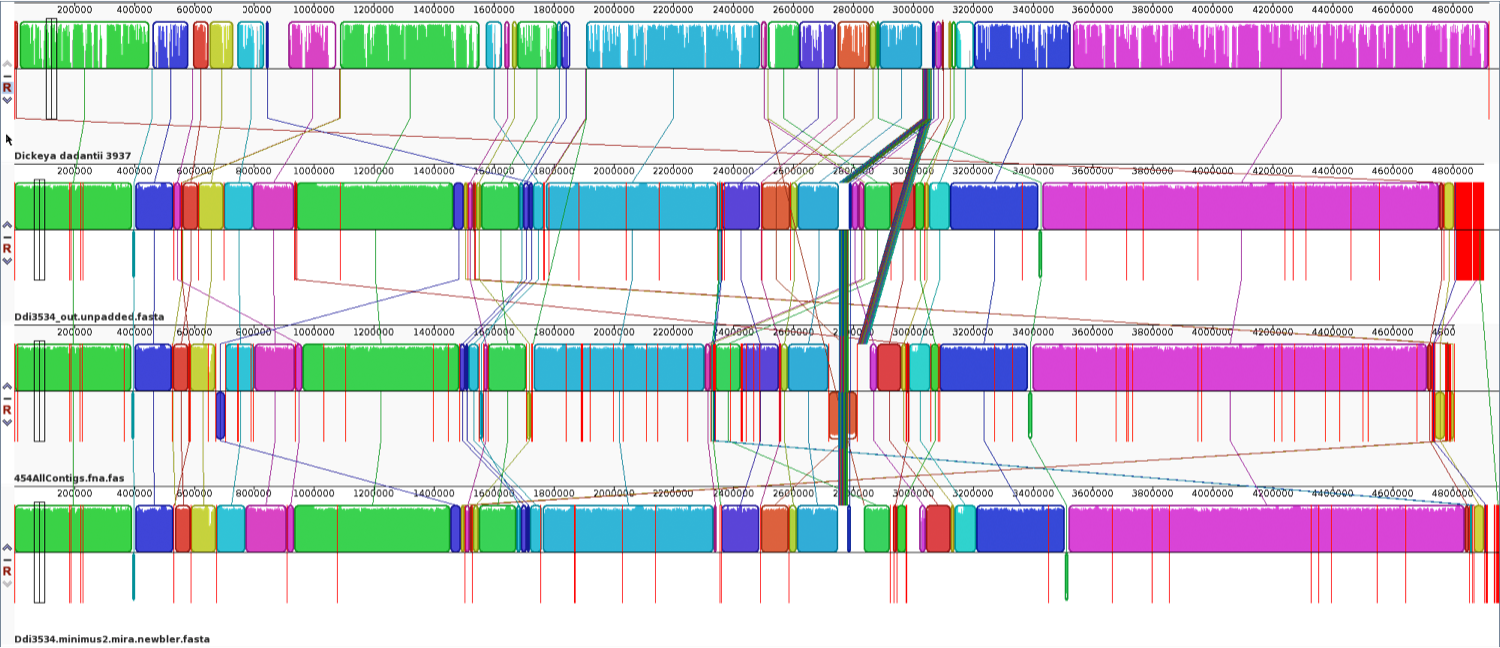
\includegraphics[width=\textwidth]{images/mauve_scaffolding}
  \end{center}    
\end{frame}

%
\begin{frame}
  \frametitle{Draft genome alignment}
  Alignment-based scaffolding:
  \begin{itemize}
    \item \textcolor{hutton_blue}{MUMmer}: \texttt{nucmer}, or \texttt{promer} (if divergent)
    \item \textcolor{hutton_purple}{MAUVE/Progressive MAUVE}: Mauve Contig Mover (MCM)
  \end{itemize}
  \begin{center}
    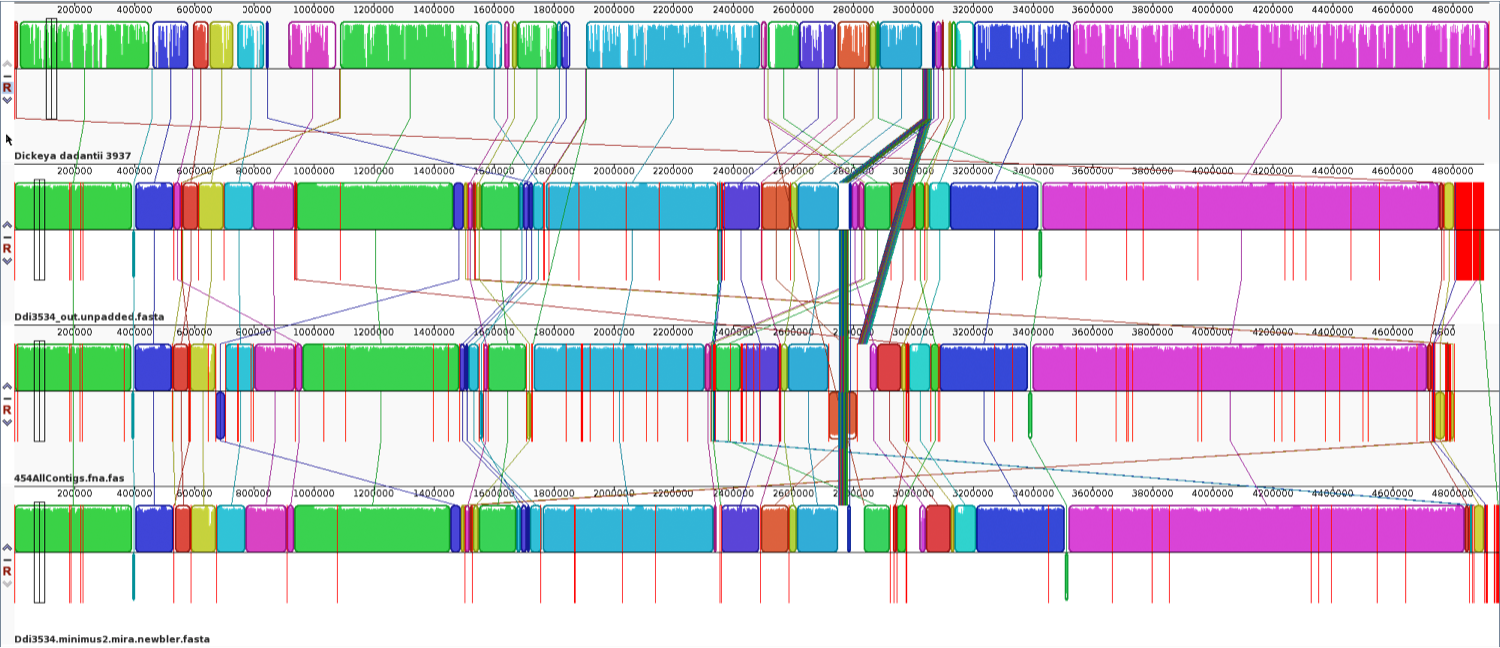
\includegraphics[width=\textwidth]{images/mauve_scaffolding}
  \end{center}    
\end{frame}

%
\begin{frame}
  \frametitle{Multiple genome alignment}
  \Large{
    \textcolor{hutton_blue}{
      \textbf{
      EXERCISE 5: \\
      {\small \href{https://github.com/widdowquinn/Teaching-2015-03-17-UoD_compgenvis/blob/master/exercises/whole_genome_alignment/whole_genome_alignments_B.md}{\texttt{whole\_genome\_alignment/whole\_genome\_alignments\_B.md}}}
      }
    }
  }
\end{frame}

%
\begin{frame}
  \frametitle{Multiple genome alignment}
  \Large{
    \textcolor{hutton_blue}{
      \textbf{
      EXERCISE 6: \\
      \texttt{ex06\_biopython\_visualisation.ipynb}
      }
    }
  }
\end{frame}

% DNA-DNA hybridisation
\begin{frame}
  \frametitle{Chromosome painting\footnote{\tiny{\href{http://dx.doi.org/10.1093/molbev/mst055}{Yahara \textit{et al}. (2013) \textit{Mol. Biol. Evol.} \textbf{30}:1454-1464 doi:10.1093/molbev/mst055}}}}
  ``Chromosome painting'' infers recombination-derived `chunks'\\
  Genome's haplotype constructed in terms of recombination events from a `donor' to a `recipient' genome\\
  \begin{center}
    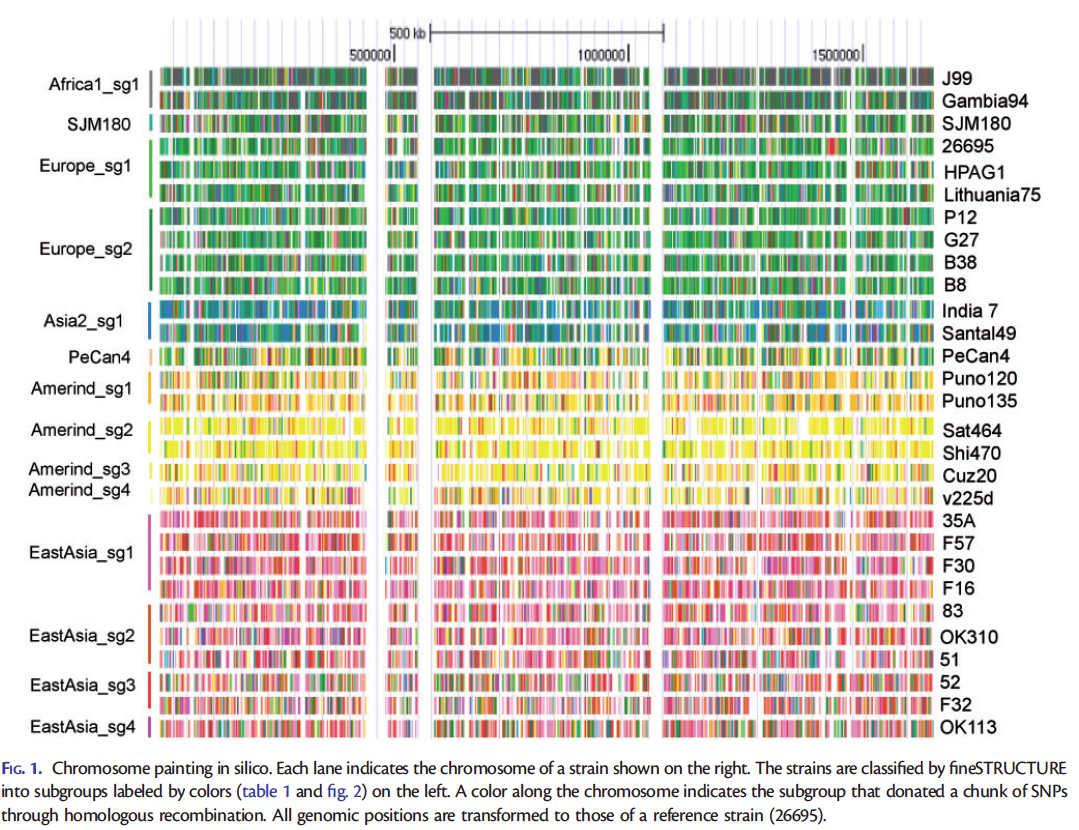
\includegraphics[width=0.7\textwidth]{images/chromosome_painting}
  \end{center}     
\end{frame}

% DNA-DNA hybridisation
\begin{frame}
  \frametitle{Chromosome painting\footnote{\tiny{\href{http://dx.doi.org/10.1093/molbev/mst055}{Yahara \textit{et al}. (2013) \textit{Mol. Biol. Evol.} \textbf{30}:1454-1464 doi:10.1093/molbev/mst055}}}}
  Recombination events summarised in a \textit{coancestry matrix}.\\
  \textit{H. pylori}: most within geographical bounds, but asymmetrical donation from Amerind/East Asian to European isolates.
  \begin{center}
    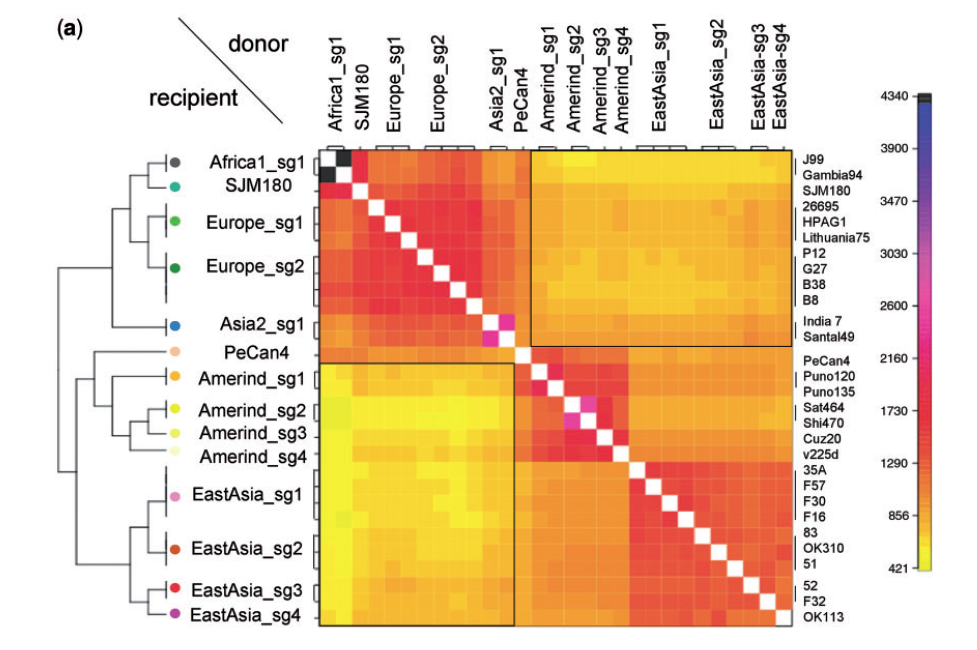
\includegraphics[width=0.75\textwidth]{images/coancestry}
  \end{center}     
\end{frame}

%
\begin{frame}
  \frametitle{Conclusions}
  \textcolor{RawSienna}{Physical and computational genome comparisons} \\
  \begin{itemize}
    \item Similar biological questions
    \item \textcolor{red}{$\therefore$ similar concepts}
  \end{itemize}  
  \textcolor{hutton_green}{Modern biology: lots of sequence data}
  \begin{itemize}
    \item Conservation $\approx$ evolutionary constraint
    \item \textcolor{hutton_blue}{Many choices of algorithms/software}
    \item \textcolor{hutton_purple}{Many choices of visualisation tools/software}
  \end{itemize}  
\end{frame}


%%%
% LICENCE FOR REUSE
%% licence.tex
%% Author: Leighton Pritchard
%% Copyright: James Hutton Institute
%% These slides describe the licence for reuse of these slides and
%% materials

%
\begin{frame}
  \frametitle{Licence: CC-BY-SA}
  By: Leighton Pritchard \\[0.5cm]
  This presentation is licensed under the Creative Commons Attribution ShareAlike license \\
  \href{https://creativecommons.org/licenses/by-sa/4.0/}{https://creativecommons.org/licenses/by-sa/4.0/}
\end{frame}

% etc
\end{document}